\chapter{Finite element discretization}
\label{chap: finite element}

In this section we present the classical variational formulation of problems \referenzaeq{eq: newton step NLP linear}, \referenzaeq{eq: LEC system new} and \referenzaeq{eq: LHC system new}. For each kind of PDE problem we give a briefly presentation of the well-posedness analysis. Finally we describe the finite element discretization. 


\section{Non Linear Poisson Equation: weak form}
\label{sec: NLP weak form}

Let us write problem \referenzaeq{eq: newton step NLP linear} in a more compact form

\begin{equation}
\label{sys: NLP general problem linearized}
\left\{
\begin{array}{rcll}
\nabla \cdot (-\epsilon \nabla \delta \varphi^k) + \sigma^k \delta \varphi^k & = &  f^k & \psp{15} in \psp{2} \Omega \\
\delta \varphi^k & = & 0 & \psp{15} on \psp{2} \Gamma_D \\
\nabla \delta \varphi ^k\cdot \vect{n} & = & 0 & \psp{15} on \psp{2} \Gamma_N
\\
\varphi^{k+1} & = & \varphi^k + \delta \varphi^k
\end{array}
\right.
\end{equation}

having set

\begin{align*}
\epsilon & = \epsilon_s \mathcal{I}_{\Omega_{Si}} + \epsilon_{ox} \mathcal{I}_{\Omega_{ox}} \\
f & = f_s \mathcal{I}_{\Omega_{Si}} + f_{ox} \mathcal{I}_{\Omega_{ox}} \\
\sigma & = \sigma_s \mathcal{I}_{\Omega_{Si}}
\end{align*}

where $\mathcal{I}_A(\vect{x})$ is equal to $1$ if $\vect{x}\in A$ and $0$ otherwise.
System \referenzaeq{sys: NLP general problem linearized} is a classical Diffusion-Reaction (DR) problem in $\Omega$, with the respect to the variable $\delta \varphi^k$. 
Now we multiply the first equation in \referenzaeq{sys: NLP general problem linearized} with a test function $v \in H^1_{\Gamma_D}$ and by integrating over all the domain we obtain

\begin{equation}
\label{eq: integration first}
- \int_{\Omega} \epsilon \Delta \delta\varphi^k  v \, d\Omega + \int_{\Omega} \sigma^{k}\delta \varphi^k v \, d\Omega = \int_{\Omega} f^{k}v \, d\Omega \psp{15} \forall v \in H^1_{\Gamma_D}(\Omega).
\end{equation}

Applying the Green-formula on \referenzaeq{eq: integration first} and then considering the boundary conditions, we get the weak formulation which reads as: find $\delta \varphi^k \in H^1_{\Gamma_D}(\Omega)$ such that

\begin{equation}
\label{eq: NLP weakformulation}
\int_{\Omega} \epsilon \nabla \delta\varphi^k \nabla v \, d\Omega + \int_{\Omega} \sigma^{k}\delta \varphi^k v \, d\Omega = \int_{\Omega} f^{k}v \, d\Omega \psp{15} \forall v \in H^1_{\Gamma_D}(\Omega)
\end{equation}

We are able to define the following bilinear form

\begin{equation}
\label{eq: bilinear form NLP linearized}
a : H^1_{\Gamma_D}(\Omega) \times H^1_{\Gamma_D}(\Omega) \rightarrow \mathbb{R}, \psp{10} a(u,v) =  \int_{\Omega} \epsilon \nabla u \nabla v \, d\Omega + \int_{\Omega} \sigma^{k}u v \, d\Omega
\end{equation}

and the linear and bounded functional

\begin{equation}
\label{eq: functional NLP linearized}
F:H^1_{\Gamma_D}(\Omega)\rightarrow \mathbb{R}, \psp{10} F(v) = \int_{\Omega} f^{k}v \, d\Omega
\end{equation}

In order to prove the existence and uniqueness of the solution, we apply the \textit{Lax-Millgram theorem} \cite{salsa:EDP} to the weak formulation \referenzaeq{eq: NLP weakformulation}.
The well-posedness is ensured by several and physical hypotesis:

\begin{itemize}
\item $\epsilon \in L^{\infty}(\Omega)$ and $\exists m$ s.t. $0 < m \leq \epsilon$ (a.e.) in $\Omega$;
\item  $\forall k \geq 0$ $\sigma^k \in L^{\infty}(\Omega)$ and $\exists m$ s.t. $0 < m \leq \sigma^k$ (a.e.) in $\Omega_{Si}$.
\end{itemize}

We define some useful quantities:

\begin{equation*}
\begin{array}{ll}
\epsilon_M = max_{\Omega} \epsilon & \epsilon_m = min_{\Omega} \epsilon \\
\sigma_M = max_{\Omega} \sigma & \sigma_m = max_{\Omega} \sigma = 0 \\
\end{array}
\end{equation*}

Take into account the above hypotesis it's possible to demonstrate:
\begin{itemize}
\item \textbf{Continuity of the bilinear form},
\begin{equation*}
\small
\begin{array}{ll}
\forall u,v \in H^1_{\Gamma_D} &\\ \\
|\int_{\Omega} \epsilon \nabla u \nabla v + \int_{\Omega} \sigma^{k}u v| 
& \leq \epsilon_{M} ||\nabla u ||_{L^2} || \nabla v ||_{L^2} +  \sigma_{M} ||u ||_{L^2} ||v ||_{L^2} 
\\
& \leq max\{\epsilon_{M}, \sigma_{M} \}  
\left( ||\nabla u ||_{L^2} || \nabla v ||_{L^2} +   ||u ||_{L^2} ||v ||_{L^2} \right)
\\
& \leq max\{\epsilon_{M}, \sigma_{M} \}  
||u ||_{H^1_{\Gamma_D}} || v ||_{H^1_{\Gamma_D}}
\end{array}
\end{equation*}

\item \textbf{Coercivity of the bilinear form,}
\begin{equation*}
\begin{array}{ll}
\forall u \in H^1_{\Gamma_D} &\\ \\
|\int_{\Omega} \epsilon \nabla u \nabla u + \int_{\Omega} \sigma^{k}u^2| 
& \geq \epsilon_{m} ||\nabla u ||_{L^2}^2  +  \sigma_{m} ||u ||_{L^2}^2 
\\
& =  \epsilon_{m} ||\nabla u ||_{L^2}^2 
\\
& = \epsilon_{m} |\nabla u |_{H^1_{\Gamma_D}}^2 
\end{array}
\end{equation*}

\item \textbf{Continuity of the functional,}
\begin{equation*}
\begin{array}{ll}
|\int_{\Omega} f^{k} v |
& \leq ||f^{(k)} ||_{L^2}||v ||_{L^2} \psp{15} \forall v \in H^1_{\Gamma_D}
\end{array}
\end{equation*}
\end{itemize}

Then we can state that $\forall k \geq 0$ there exists a unique solution of the linearized Non Linear Poisson equation.

\section{Continuity Equations: weak form}

Without loss of generality we can consider only the electron continuity equation. System \referenzaeq{eq: LEC system new} is a classical diffusion-advection-reaction (DAR) problem written in conservative form. With a suitable change of variables we are able to treat these PDE's equations likewise the linearized Non Linear Poisson equation in the previous section. Consider the Slotboom variable \referenzaeq{eq: un slotboom}, we can rewrite system \referenzaeq{eq: LEC system new} as:

\begin{equation}
\label{eq: system continuity equation}
\small
\left\{
\begin{array}{rcll}
 \nabla \cdot \left( - q D_n e^{(\varphi^{i}/V_{th})}\nabla u_n \right) + \sigma_n^{i-1} e^{(\varphi^{i}/V_{th})} u_n& = & f^{i-1}  & \psp{15} in \psp{2} \Omega_{Si} \\
u_n & = &  n_D e^{(-\varphi^{i}/V_{th})} & \psp{15} on \psp{2} \Gamma_{D,Si} \\
\nabla u_n \cdot \vect{n} & = & 0 & \psp{15} on \psp{2} \Gamma_{N,Si}
\end{array}
\right.
\end{equation}

We can easily obtain the weak formulation as section \ref{sec: NLP weak form}. Therefore the weak formulation of the Electron Continuity equation is: find $u_n \in H^1_{\Gamma_{D,Si}}(\Omega)$ such that:

\begin{equation}
\footnotesize
\label{eq: LEC weakformulation}
\int_{\Omega_{Si}}  q D_n e^{(\varphi^{i}/V_{th})} \nabla u_n \nabla v \, d\Omega + \int_{\Omega_{Si}} \sigma_n^{i-1} e^{(\varphi^{i}/V_{th})} u_n v \, d\Omega = \int_{\Omega_{Si}} f^{i-1}v \, d\Omega \psp{10} \forall v \in H^1_{\Gamma_{D,Si}}
\end{equation}


The existence and uniqueness of the unknown variable $u_n$ ensures the same properties on $n$, thanks to the univocal relation between $u_n$ and $n$.
Further hypotheses on the coefficients $\forall i\geq 0$:
\begin{itemize}
\item $q D_n e^{(\varphi^{i}/V_{th})} \in L^{\infty}(\Omega_{Si})$ and $\exists m$ s.t. $0 < m \leq q D_n e^{(\varphi^{i}/V_{th})}$ (a.e.) in $\Omega_{Si}$;
\item  $\sigma_n^{i-1} e^{(\varphi^{i}/V_{th})} \in L^{\infty}(\Omega_{Si})$ and $\exists m$ s.t. $0 < m \leq \sigma_n^{i-1} e^{(\varphi^{i}/V_{th})}$ (a.e.) in $\Omega_{Si}$.
\end{itemize}

We define the relative bilinear form

\begin{equation}
\label{eq: bilinear form LEC}
a(u,v) =  \int_{\Omega_{Si}}  q D_n e^{(\varphi^{i}/V_{th})} \nabla u_n \nabla v \, d\Omega + \int_{\Omega_{Si}} \sigma_n^{i-1} e^{(\varphi^{i}/V_{th})} u_n v \, d\Omega
\end{equation}

and the linear and bounded functional

\begin{equation}
\label{eq: functional LEC}
F(v) = \int_{\Omega_{Si}} f^{i-1}v \, d\Omega
\end{equation}

Now the well-posedness of this problem is ensured just by following the procedure of section \ref{sec: NLP weak form}.



\section{Numerical approximation}
\label{sec: Numerical approximation}


In this section we introduce the classical Galerkin's method to approximate the weak formulation on $\Omega$. Each weak formulation could be represented in a more compact and generic form as, find $u \in V$ such that

\begin{equation}
a(u,v) = F(v) \psp{10} \forall v \in V
\end{equation}

where $V$ is the space of admissible functions, e.g. $H^1_{\Gamma_D}(\Omega)$, $H^1_{\Gamma_{D,Si}}(\Omega_{Si})$.
 Let us introduce $V_h$ which is a family of finite-dimensional subspace of $V$, depending by a positive parameter $h$, such that

\begin{equation}
V_h \subset V, \psp{5} dim V_h < \infty \, \forall h>0
\end{equation}

The \textit{Galerkin's problem} reads as, find $u_h\in V_h$ such that:

\begin{equation}
\label{eq: general galerkin problem}
 a(u_h,v_h) = F(v_h) \psp{3} \forall v_h \in V_h
\end{equation}

Let be $\mathcal{T}_h$, a finite partition of $\Omega$, and $K$ a generic element of $\mathcal{T}_h$ such that  $\bar{\Omega} =  \bigcup \bar{K}$. In this case the parameter $h$ refers to the characteristic dimension of the elements $K$.
Let us introduce the general finite element spaces of the polynomial element-wise functions:

\begin{equation}
X^r_h(\Omega) := \{v_h \in C^0(\bar{\Omega}): v_h|_K\in \mathbb{P}_r,\forall K \in \mathcal{T}_h \}
\end{equation}

and the relative space where functions vanish on boundaries

\begin{equation}
X^r_{h,\Gamma_D}(\Omega)  := \{ v_h \in X^r_h: v_h|_{\Gamma_D} = 0 \} .
\end{equation}

If $\Omega \in \mathbb{R}^3$ we have:
\begin{equation}
\small
\label{eq: dimensione polinomi}
dim\mathbb{P}_r := \dfrac{(r+1)^3}{2} + \dfrac{(r+1)^2}{2} + \dfrac{r(r+1)(2r+1)}{12} - \dfrac{r(r+1)^2}{2} - \dfrac{r(r+1)}{4}
\end{equation}

More precisely we approximate $H^1_{\Gamma_D}(\Omega)$ with $X^1_{h,\Gamma_D}(\Omega)$ and $H^1_{\Gamma_{D,Si}}(\Omega_{Si})$ with $X^1_{h,\Gamma_{D,Si}}(\Omega_{Si})$. Therefore accordingly with \referenzaeq{eq: dimensione polinomi} we have

\begin{align*}
dim \mathbb{P}_1 & = 4 \\
dim X^1_h & = N_h \\
dim X^1_{h,\Gamma_D} & = N_h - N_g
\end{align*}

where $N_h$ is the number of vertices of the partition $\mathcal{T}_h$ and $N_g$ are the number of vertices lie on Dirichlet boundaries.

We denote by $\{ \psi_j \}_{j=1}^{N_h} $ the Lagrangian basis of the space $X^1_{h}$. Naturally  as $u_h \in X^1_{h}$ there are $u_j \in \mathbb{R}$ with $j=1,\, ... \,, N_h$ such that:


\begin{equation}
u_h = \sum_{j=1}^{N_h} u_j \psi_j
\end{equation}

Because each functions of $V_h$ is a linear combination of $\psi_i$, we can test equation \referenzaeq{eq: general galerkin problem} only for each basis function rather than $\forall v_h \in V_h$. The result of the complete discretization is find $u_j$, with $j = 1, \, . \, . \, . \, , \, N_h$ such that:

\begin{equation}
\sum_{j=1}^{N_h}u_ja(\psi_j,\psi_i) = F(\psi_i) \psp{10} \forall i = 1, \, . \, . \, . \, , \, N_h
\end{equation}

In order to implement this routine it's useful make explicit the subdivision of the bilinear form on the element of the partition $\mathcal{T}_h$:

\begin{equation}
\label{eq: sistema algebrico in sommatoria}
\sum_{j=1}^{N_h}u_j\sum_{K\in \mathcal{T}_h}a_K(\psi_j,\psi_i) = \sum_{K\in \mathcal{T}_h}F_K(\psi_i) \psp{10} \forall i = 1, \, . \, . \, . \, , \, N_h
\end{equation}


\subsection{Geometrical discretization}

Each element $K\in \mathcal{T}_h$ is set as a tetrahedral of volume $|K|$; Let $\delta>0$ be a constant such that:

\begin{equation}
\label{eq: mesh regular condition}
\dfrac{h_K}{\rho_K} \leq \delta \psp{15} \forall K \in \mathcal{T}_h
\end{equation}

where $h_k=diam(K)=max_{x,y\in K}|x-y|$ and $\rho_K$ is the diameter of the sphere inscribed in the tetrahedral $K$. Condition \referenzaeq{eq: mesh regular condition} is the so called \textit{mesh regularity condition} \cite{quarteroni:modnum} and it ensures an istoropic partition.
We denote with $\mathcal{E}_h$, $\mathcal{V}_h$ and $\mathcal{F}_h$ the set of all the edges, vertices and faces  
of $\mathcal{T}_h$ respectively, and for each $K\in \mathcal{T}_h$ we denote by $\partial K$ and $\vect{n}_{\partial K}$ the boundary of the element and its outward unit normal.
  
We note that $\mathcal{T}_h$ is built such that every $K$ belongs to a single region, while it is possible that vertices belong to different regions.  
 
 \subsection{Linearized Non Linear Poisson equation}

As regards the linearized NLP equation we have:
\begin{equation}
a(\psi_j,\psi_i)  = \int_{\Omega} \epsilon \nabla \psi_j \nabla \psi_i \, d\Omega + \int_{\Omega} \sigma^{k}\psi_j \psi_i \, d\Omega 
\end{equation}
and the relative restriction on element $K$ is
\begin{equation}
\label{eq: bilinear local discrete}
a_K(\psi_j,\psi_i)  = \int_{K} \epsilon \nabla \psi_j \nabla \psi_i \, dK + \int_{K} \sigma^{k}\psi_j \psi_i \, dK
\end{equation}

Equation \referenzaeq{eq: bilinear local discrete} it's formed by two distinct contributions, the former identifies the diffusive contribution and generates the so called \textit{stiffness matrix}, while the latter refers to the reaction and generates the \textit{mass matrix}.

The coefficient $\epsilon$ is a piece-wise constant function, which changes on different material regions. Therefore $\epsilon$ is constant over each elements and integral in \referenzaeq{eq: bilinear local discrete} become easier.

As a consequence of choose the discrete space $X^1_{h}$,  we can't expect a better priori estimation error on the solution, than the first order in $||\cdot||_{1,\Omega}$ respect the characteristic discretization step $h_K$ \cite{quarteroni:modnum}. This implies that is not necessary and useful the use of an high order quadrature, and the trapezoidal rule is enough accurate. 
The main consequence of using trapezoidal quadrature rule is that extra-diagonal elements of the mass-matrix disappear.
This technique is well known as \textit{lumping procedure} applied on the mass-matrix.

Finally the contributions of the local system matrix $A_K^k$ is:

\begin{equation}
[A_K^k]_{ij}  = \epsilon_K
L_{ij}
+
\dfrac{|K|}{4} \sigma^k_i
\end{equation}

having set

\begin{equation}
\begin{array}{rcl}
L_{ij} & \simeq & \int_K \nabla \psi_i  \nabla \psi_j \, d\Omega \\ \\
\sigma^k_i & =  &\sigma^k(\vect{x}_i)
\end{array}
\end{equation}

The construction of the right hand side of \referenzaeq{eq: sistema algebrico in sommatoria} with trapezoidal rule is:

\begin{equation}
[F_K]_i^k =  f^k_i |K| / 4 \simeq \int_{\Omega} f^k \psi_i \, d\Omega 
\end{equation}

The local contributions of each element $K$ must be assembled in the global matrix $A$: let $I$ be the global index of a generic vertex belonging to the partition $\mathcal{T}_h$, we denote by $\mathcal{J}_K: \mathcal{V}_{\mathcal{T}_h} \rightarrow \mathcal{V}_{K}$ the map which connects $I$ to its corresponding local index $i=1, \, . \, . \, . \, , 4$ in the element $K$. Then we have 

\begin{equation}
A_{IJ}^k = \sum_{\substack{\forall K \in \mathcal{T}_h s.t. \\ \mathcal{J}_K(I),\mathcal{J}_K(J) \subset \mathcal{V}_K}}
 [A_K]_{ij}^k
\end{equation}

analogously for the force term $\vect{b}^{(k)}$:

\begin{equation}
b_{I}^k = \sum_{\substack{\forall K \in \mathcal{T}_h s.t. \\ \mathcal{J}_K(I) \subset \mathcal{V}_K}}
 [F_K]_{i}^k
\end{equation}

Once we have built the global matrix $A^k$ and the global vector $\vect{b}^k$ we need to take into account the essential boundary conditions. In fact the displacement formulation is a primal formulation which forces Dirichlet boundary condition in a strong way. Therefore we have to modify the algebraic system. We choose the \textit{diagonalization} technique which does not alter the matrix pattern nor introduce ill-conditioning for the system.  Let $i_D$ be the generic index of a Dirichlet node, we denote by $[\delta \varphi_{D}]_i$ (which in this case is equal to zero) the known value of the solution $\delta \varphi $ at the node. We consider the Dirichlet condition as an equation of the form $a [\delta \varphi]_i = a [\delta \varphi_{D}]_i$, where $a\neq 0$ is a suitable coefficient. In order to avoid degrading of the global matrix condition number, we take $a$ equal to the diagonal element of the matrix at the row  $i_D$.

Finally we have completed the discretization of (Step 1), which reads as follows:

\begin{equation}
\label{eq: NLP discretizated}
\left\{
\begin{array}{rcl}
A^k\vect{\delta \varphi}^k & = & \vect{b}^k \\
\vect{\varphi}^{k+1} & = & \vect{\varphi}^k +  \vect{\delta \varphi}^k 
\end{array}
\right.
\end{equation}

As every iteration procedure, problem \referenzaeq{eq: NLP discretizated} needs a suitable convergence break criterion. A good method is based on checking the satisfaction of the fixed point equation \referenzaeq{eq: abstract problem fully} by the $k$-th solution. In this case the inner loop of the Gummel Map reads as: given a tolerance $toll>0$ solve problem \referenzaeq{eq: NLP discretizated} untill:
\begin{equation}
||\vect{b}(\varphi^{k+1})||_2 > toll
\end{equation}

where $||\cdot ||_2$ is the usual Euclideian norm for a vector.
\subsubsection{Damping}

Nevertheless the theorem \referenzaeq{theorem: newton convergence}, the system \referenzaeq{eq: NLP discretizated} may be affected by difficulties on the convergence velocity.
The main problem associated with the classical Newton method is the tendency to overestimate the length of the present correction step. This phenomenon is frequently indicated as \textit{overshoot}. In the case of the semiconductor equations this overshoot problem has often been treated by simply limiting the size of the correction vector ($\delta \varphi$) determined by Newton's method. The usual established modifications to avoid overshoot are given by the follow formulations:


\begin{align}
\tilde{A}(\varphi_k)&=\dfrac{1}{t_k}A(\varphi_k) \label{eq: NLP mod used}
\end{align}

$t_k$ is a properly chosen positive parameter: for $t_k=1$ the modified Newton method reduces to the classical Newton method. We have now to deal with the question how to choose $t_k$ such that the modified Newton method exhibits superior convergence properties compared to the classical Newton method.
For the case \referenzaeq{eq: NLP mod used} there's a simple criterion suggested by Deuflhard \cite{DefulhardDamp}. $t_k$ is taken from the interval $(0,1]$ in such a manner that for any norm,

\begin{equation}
\label{eq: extended criterion}
||A(\varphi_k)^{-1}\vect{b}(\varphi_k-t_kA(\varphi_k)^{-1}\vect{b}(\varphi_k))||<||A(\varphi_k)^{-1}\vect{b}(\varphi_k)||
\end{equation}

Condition \referenzaeq{eq: extended criterion} guarantees that the correction of the k-th iterate is an improved approximation to the final solution, in other words the residual norm can only descents.
This condition is hardly to be evaluated as the presence of the inverse system matrix. If the Jacobian matrix is factored into triangular matrices the evaluation of the argument of the norm on the left hand side of \referenzaeq{eq: extended criterion} is reduced to a forward and backward substitution and the evaluation of $\vect{b}(\varphi)$. Although we use an iterative method (BCG solver based on \cite{NumericalRecipes}) which implies serious difficulties to the application of the above criterion. Another valid possibility is to use the main diagonal of $A(\varphi_k)$, denoted as $D(\varphi_k)$:
\begin{equation}
\label{eq: easy criterion}
||D(\varphi_k)^{-1}\vect{b}(\varphi_k-t_kD(\varphi_k)^{-1}\vect{b}(\varphi_k))||<||D(\varphi_k)^{-1}\vect{b}(\varphi_k)||
\end{equation}

This criterion has been adopted in our code. However the value to use for $t_k$ is a question of trial and error. Frequently the following sequence is used:

\begin{align}
t_k & = \dfrac{1}{2^i} \\
t_k & = \dfrac{1}{2^{\dfrac{i(i+1)}{2}}}  
\end{align}

where $i$ is the subiterations of damping reached when \referenzaeq{eq: easy criterion} is satisfied. Close to the solution, \referenzaeq{eq: extended criterion} (and so \referenzaeq{eq: easy criterion}) will be satisfied with $t_k=1$ so that the convergence properties of the classical Newton method are recovered.
 

\begin{figure}[!h]
\centering

\subfloat[][\emph{Non Linear Poisson residual: damping benefit prodedure.}]
{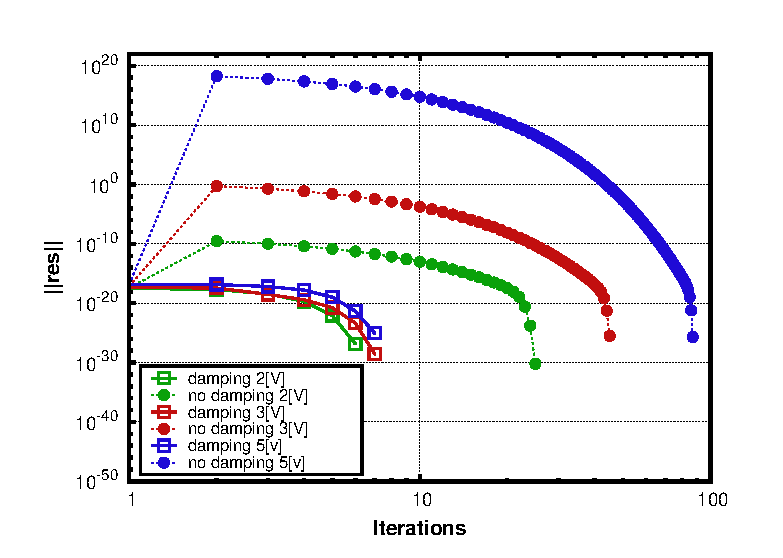
\includegraphics[height=7cm]{FiniteElementDiscretization/NLPconver/NLPconvergence.eps}}

\subfloat[][\emph{$t_k$ parameter.}]
{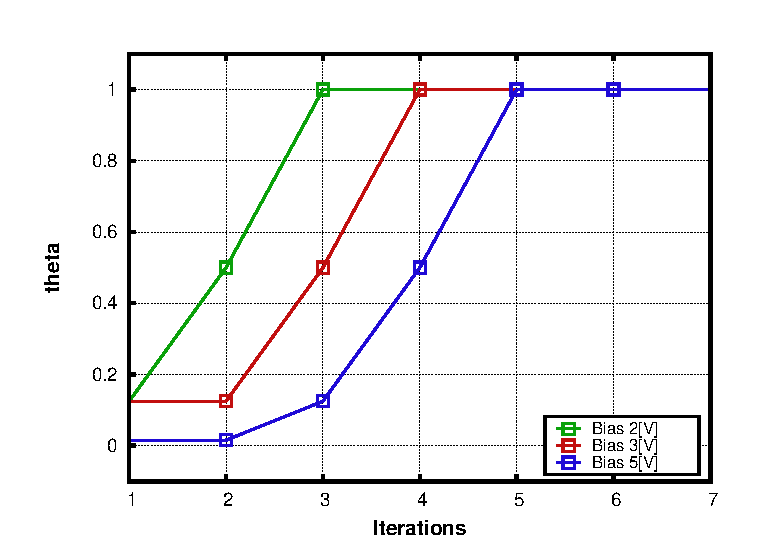
\includegraphics[height=7cm]{FiniteElementDiscretization/NLPconver/NLPtheta}}

\caption{(a) Number of iteration against residual for different voltages in a diode test case. (b) Magnitude of the damping parameter $t_k$.}

\end{figure}




\subsection{Continuity equations}
\label{sec: continuity equations}

As regards the \referenzaeq{eq: system continuity equation} equation we can write the bilinear form as

\begin{equation}
\label{eq: weak formulation displacement}
a(u,v) =  \int_{\Omega_{Si}}  q D_n e^{(\varphi^{i}/V_{th})} \nabla \psi_j \nabla \psi_i \, d\Omega + \int_{\Omega_{Si}} \sigma_n^{i-1} e^{(\varphi^{i}/V_{th})} \psi_j \psi_i \, d\Omega
\end{equation}

Even if this form guarantees an easily analysis of well-posedness, the choice of using Slotboom variables $u_n$ and $u_p$ causes the onset of overflow problems due to the evaluation of $exp(\varphi/V_{th})$, which can be a rapidly varying function according to the behaviour of the potential $\varphi$.

Therefore special care has to be taken in the treatment of the diffusion coefficient. In view of further discussions of this issue, we introduce some useful notation. For each set $S \subset \Omega$ having measure $|S|$, we introduce the following averages of a given function $g$ that is integrable on $S$:

\begin{equation*}
\mathcal{M}_S(g) = \dfrac{\int_S g \, dS}{|S|} \psp{15} \mathcal{H}_S = (\mathcal{M}_S(g^{-1}))^{-1} 
\end{equation*}

Notice that $\mathcal{M}_S$ is the usual integral average, while $\mathcal{H}_S$ is the \textit{harmonic average}. It is well-known that the use of the harmonic average provides a superior approximation performance \cite{BabuskaMixMet}.


The weak form \referenzaeq{eq: weak formulation displacement}  is the result of a displacement approach which is the most classical way of setting these problems, although different variational formulations and therefore different finite element approximations may be used, like a primal mixed approach (PM) (for a more complete treatment see \cite{Zikatanov:EAFE} and \cite{TesiDotDeFalco}).  First of all it's convenient to reformulate problem \referenzaeq{eq: LEC system new} by using the relation \referenzaeq{eq: un slotboom} and \referenzaeq{eq: Jn slotboom} in a more generic form. This yields the following equivalent form

\begin{equation}
\label{eq: LEC system slotboom generic}
\begin{cases}
\nabla \cdot (\vect{J}_n(n) ) +\sigma n = f & in \psp{3} \Omega_{Si}
 \\
 \vect{J}_n = qD_n e^{(\varphi/V_{th})} \nabla (e^{(-\varphi/V_{th})}n) & in \psp{3} \Omega_{Si}\\
n = n_D & on \psp{3} \Gamma_{D,Si}
 \\
 \vect{J}_n \cdot \vect{n} = 0 & on \psp{3} \Gamma_{N,Si}
\end{cases}
\end{equation}

We report here the weak formulation of \referenzaeq{eq: LEC system slotboom generic} which is well investigated in \cite{TesiDotDeFalco}, find $\vect{J}_n \in [L^2(\Omega)]^d$ and $n \in H^1_{\Gamma_{D,Si}}(\Omega)$ such that

\begin{align}
- \int_{\Omega_{Si}} \vect{J}_n\cdot \nabla v \, d\Omega + \int_{\Omega_{Si}} \sigma n v \, d\Omega = \int_{\Omega_{Si}} f v \, d\Omega \psp{10} \forall v \in H^1_{\Gamma_{D,Si}}(\Omega)
\label{eq: weak form PM1} \\
\int_{\Omega_{Si}} (qD_n e^{(\varphi/V_{th})})^{-1} \vect{J}_n\cdot \vect{q} \, d\Omega + \int_{\Omega_{Si}} \nabla(e^{(\varphi/V_{th})}n) \cdot \vect{q} \, d\Omega = 0 \psp{10} \forall \vect{q} \in [L^2(\Omega)]^d \label{eq: weak form PM2} 
\end{align}

In order to approximate $[L^2(\Omega)]^d$ we introduce a new discrete space

\begin{equation}
\Sigma_h := \left\{   \vect{q}_h \in  [L^2(\Omega)]^d : \vect{q}|_{K} \in [\mathbb{P}_0]^d \forall K \in \mathcal{T}_h\right\}
\end{equation} 

as usual $d$ is the dimension of $\Omega$ and if $d=3$, $\vect{q}_h$ is characterized for every $K \in \mathcal{T}_h$ by the triplet

\begin{equation}
\label{eq: form of qh}
\vect{q}^h_{1,2,3} = \left\{ \begin{bmatrix} 1 \\ 0 \\ 0 \end{bmatrix}  \begin{bmatrix} 0 \\ 1 \\ 0 \end{bmatrix}  \begin{bmatrix} 0 \\ 0 \\ 1 \end{bmatrix}  \right\}
\end{equation}

Therefore \referenzaeq{eq: weak form PM1} and \referenzaeq{eq: weak form PM2} can restricted on a generic element $K$ and the related bilinear form reads

\begin{equation}
\label{eq: LEC discretized general}
\left\{
\begin{array}{rcl}
a_h^K(n_h,v_h) & = & \int_{K}\vect{ J}_{n,h}^K(n_h) \nabla v_h \, dK + \int_{K} \sigma n_h v_h \, dK 
\\
\\
F(v_h)^K & = & \int_K f v_h \, dK
\\
\\
\vect{J}_{n,h}^K & = & D_K(qD_n e^{(\varphi/V_{th})}) \nabla  (e^{(-\varphi / V_{th})}n_h)
\end{array}
\right.
\end{equation}

where $D_K \in \mathbb{R}^{3\times 3}$ is the element stiffness matrix. Several treatments may be performed on this matrix

\begin{equation}
\label{eq: vari diffusion coeff}
 D_K(qD_n e^{(\varphi/V_{th})}) = 
 	\begin{cases}
		  \mathcal{M}_K(qD_n e^{(\varphi/V_{th})}) \\
		  \mathcal{H}_K(qD_n e^{(\varphi/V_{th})}) \\
 		  \dfrac{1}{|K|}\sum_{i=1}^6 \mathcal{H}_{e_i}(qD_ne^{(\varphi/V_{th})}) |e_i| s_i \vect{t}_i \vect{t}_i^T
 		 \end{cases}
\end{equation}


These different approaches in the computation of the average of the diffusion coefficient are responsible for the quite different numerical perfomance of the relative methods.
We already presented the standard average and the armonic average and we discussed briefly the advantages of them. 
The latter equation in \referenzaeq{eq: vari diffusion coeff} introduces an exponentially treatment of the diffusion coefficient along each edge of the boundary $\partial K$ of the subdomain $K$. 

Considering that along the edges the approximate flux density can be written as a function of its tangential components. We have for each edge $e_i$, the tangential component of $J_h^K(n_h)$

\begin{align*}
j_{e_i}  & =   \mathcal{H}_{e_i} \dfrac{\delta_i(e^{-\varphi /V_th}n_h)}{|e_i|} = \mathcal{H}_{e_i} \nabla (e^{-\varphi / V_{th}}n_h) \vect{t}_i \\
& =  \mathcal{H}_{e_i}(qD_n e^{(\varphi/V_{th})}) \dfrac{\mathcal{B}(\delta_i(\varphi / V_{th}))n_{h,k} -  \mathcal{B}(-\delta_i(\varphi / V_{th}))n_{h,j}}{|e_i|}
\end{align*}

where 

\begin{equation}
\delta_i(\varphi / V_{th}) = \dfrac{\varphi_k - \varphi_j}{V_{th}} = 2 \dfrac{(\vect{E}_K\cdot \vect{t}_{e_i}) |e_i|}{2\mathcal{H}_{e_i}(qD_n e^{(\varphi/V_{th})}) } = 2 \gamma_i
\end{equation}

\begin{equation}
\mathcal{B}(z) = \left\{ \begin{array}{cl}
\dfrac{z}{e^z-1} & z \neq 0
\\
1 & z = 0
\end{array}
\right.
\end{equation}

being $\vect{E}_K$ the relative electric field on $K$ and $|\gamma_i|$ the P\`eclet number associated with the edge $e_i$. 
From \referenzaeq{eq: LEC discretized general} we immeditaly obtain:

\begin{equation}
\label{eq: exp fitted flux}
\vect{J}_h^K = \dfrac{1}{|K|}\sum_{i=1}^6 |e_i| s_i j_{e_i} \vect{t}_i 
\end{equation}

Furthermore having defined the flux vector over $K$ in the form \referenzaeq{eq: exp fitted flux}, it is possible to construct a fimily of Galerkin finite element approximations for the continuity equations by a proper choice of the quantities $j_{e_i}$ (e.g. upwind techniques). 




\subsubsection{The discretization scheme}

Given the choice for $j_{e_i}$ and replacing the equation for $\vect{J}_h^K$ in the bilinear form \referenzaeq{eq: LEC discretized general}, we can compute the local system matrix as

\begin{equation}
\Phi_K  = 
{
\tiny 
\left[
\begin{array}{cccc}
- \left( \begin{array}{c}
a_{e12}\mathcal{B}_{12}L^K_{21} + \\
a_{e13}\mathcal{B}_{13}L^K_{31} + \\
a_{e14}\mathcal{B}_{14}L^K_{41}
\end{array} \right)

& a_{e12}\mathcal{B}_{12}L^K_{21} 
& a_{e13}\mathcal{B}_{13}L^K_{31}
& a_{e14}\mathcal{B}_{14}L^K_{41}
\\

%-----------------------------
a_{e21}\mathcal{B}_{21}L^K_{12}
&
- \left( \begin{array}{c}
a_{e21}\mathcal{B}_{21}L^K_{12} + \\
a_{e23}\mathcal{B}_{23}L^K_{32} + \\
a_{e24}\mathcal{B}_{24}L^K_{42}
\end{array} \right)
& a_{e23}\mathcal{B}_{12}L^K_{32}
& a_{e24}\mathcal{B}_{12}L^K_{42}
\\

%-----------------------------
a_{e31}\mathcal{B}_{31}L^K_{31}
& a_{e31}\mathcal{B}_{32}L^K_{32}
&
- \left( \begin{array}{c}
a_{e31}\mathcal{B}_{31}L^K_{31} + \\
a_{e32}\mathcal{B}_{32}L^K_{32} + \\
a_{e34}\mathcal{B}_{34}L^K_{34}
\end{array} \right)

&a_{e34}\mathcal{B}_{34}L^K_{34}
\\

%-----------------------------
a_{e41}\mathcal{B}_{41}L^K_{41}
& a_{e42}\mathcal{B}_{42}L^K_{42}
&a_{e43}\mathcal{B}_{43}L^K_{43}
&
- \left( \begin{array}{c}
a_{e41}\mathcal{B}_{41}L^K_{41} + \\
a_{e42}\mathcal{B}_{42}L^K_{42} + \\
a_{e43}\mathcal{B}_{43}L^K_{43}
\end{array} \right)

\end{array}
\right]
}
\end{equation}

\begin{equation}
\label{eq: matrice continuità}
A_K = \Phi_K + \dfrac{|K|}{4} diag (\sigma)
\end{equation}

\begin{equation}
\vect{F}_K = \dfrac{|K|}{4} (f_1,f_2,f_3,f_4)^T
\end{equation}

denoting by  $\mathcal{B}_{ij}$ the Bernoulli function applied to the potential difference between node $j$ and node $i$.

The discretization scheme just presented is well known as \textit{Edge Averaged Finite Elements} (EAFE) and it's particularly suitable for problems with  highly variable coefficient. Furthermore this approach has several good properties, e.i. in 2D simulation if $\mathcal{T}_h$ is a Delauny partition the system matrix is an \textit{M-matrix} \cite{BankMmatrixEAFE}. The main consequence of this statement is that the solution could satisfy the \textit{Discrete Maximum Principle}. This is a notable property which implies that no negative concentrations are admitted. Unfortunately this property is not anymore valid in 3D framework, indeed the Delauny condition of the mesh is not sufficient to guarantee that the system matrix is an M-matrix. A more general condition is presented in \cite{ZikatanovXu}.

\begin{Teorema}[Zikatanov condition]
The system matrix of the EAFE scheme is an M-matrix if and only if for any fixed edge E of the partition $\mathcal{T}_h$ the following inequality holds:

\begin{equation}
\label{eq: mesh delaunay condition}
\omega_E = \dfrac{1}{n(n-1)} \sum_{T\supset E} |k_E^T|cot\theta_E^T \geq 0,
\end{equation}

where $n$ is the dimension, $\sum_{T \supset E}$ means summation over all simplexes $T$ containing $E$, $\theta_E^T$ is tha angle between the faces $f_i$, $f_j \in \mathcal{T}_h$ such that $f_i \bigcap f_j = E$  and $k_E^T$ is the edge in $T$ which doesn't share any verticies with $E$.
\end{Teorema}

\begin{Osservazione}
For $n=2$ the condition \referenzaeq{eq: mesh delaunay condition} means that the sum of the angles opposite to any edge is less than or equal to $\pi$, this condition implies that the partition is a Delaunay triangulation.
\end{Osservazione}

\begin{Osservazione}
Condition \referenzaeq{eq: mesh delaunay condition} highlights that in order to satisfy the discrete maximum principle, a partion without obtuse angles is preferable.
\end{Osservazione}

We remark that presently meshing algorithm are oriented to care about the minimum angle of the elements, rather than the maximum, resulting that obtain a mesh which satisfied the condition \referenzaeq{eq: mesh delaunay condition} it's a really difficult task. 

\figref{fig: cubo zikatanov} shows a simple partition of a cube performed with the Synopsis tool SNMESH. For every element we evaluated how many edges don't satisfy the condition \referenzaeq{eq: mesh delaunay condition}.
It's clear that there are a lot of edges which don't fulfill the condition and a precise pattern can't be individuated. When several bad edges belong to a single element we can indentify the presence of many obtuse angles.

In order to avoid this problem some alternative solutions are proposed in the literature, like the \textit{Orthogonal Subdomain Collocation method} \cite{OSCputticorded}, but also this approach is not definitely. 

Therefore in presence of negative concentration the most used technique during 3D numerical simulation is the increasing of the degree of freedom in the problematic regions, which often are the ones where the carrier density decrease.



\begin{figure}[!b]
\centering
{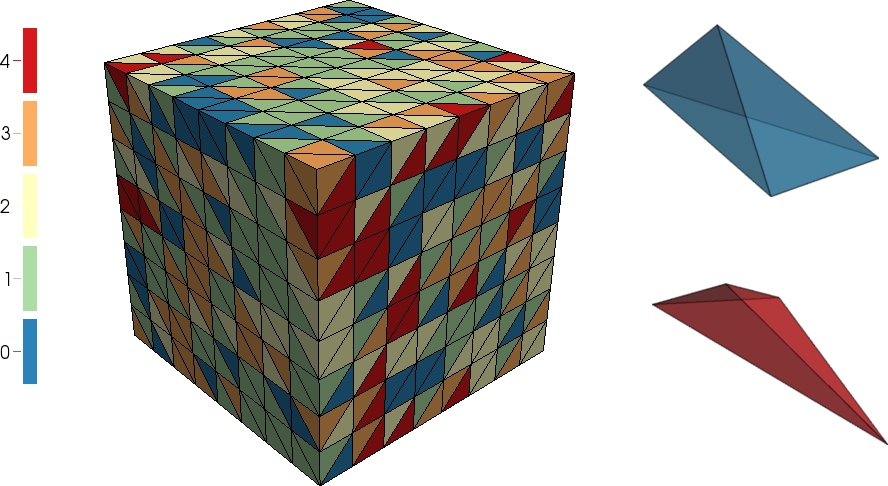
\includegraphics[width=0.75\textwidth , height = 5.5cm]{FiniteElementDiscretization/CuboElementi.png}}
\caption{Evaluation of the Zikatanov condition over a simple partition. Red elements doesn't satisfy condition  \referenzaeq{eq: mesh delaunay condition} over four edges while blue elements fully accomplished the criterion.}
\label{fig: cubo zikatanov}
\end{figure}

%\textcolor{red}{Vale la seguente uguaglianza?}
%\begin{equation}
%L_{ij} = s_{ij} \vect{t}_{ij} \cdot \nabla \psi_i
%\end{equation}